\documentclass{report}
\usepackage[landscape]{geometry}
\usepackage{longtable}
\usepackage{tabularx}
\usepackage[inline]{enumitem}
\usepackage{tikz}
\usetikzlibrary{calc,shapes, positioning,arrows}

\usepackage{bibleref}

\usepackage{minted}
\usepackage{listings}
\newcommand{\mi}[1]{\lstinline{#1}}

\makeatletter
\newenvironment{python}{%
  \VerbatimEnvironment
  \minted@resetoptions
  \setkeys{minted@opt}{}
      \begin{VerbatimOut}{\jobname.pyg}}
{%
      \end{VerbatimOut}
      \minted@pygmentize{python}
      \DeleteFile{\jobname.pyg}}
\makeatother

\usepackage{multicol}

%\usepackage[usenames, dvipsnames]{color}
%\newcommand{\fixme}[1]{{#1}}

\title{Work flow with gcdata.sqlite and several Python scripts}
\author{Grietje Commelin}

\begin{document}
\maketitle

\noindent
In this document I try to explain the work flow that I follow to gather, improve and use data about participant references by running Python scripts on the ETCBC database and my own gcdata.sqlite.\\
Data is indicated with red frames, and scripts with blue ones.

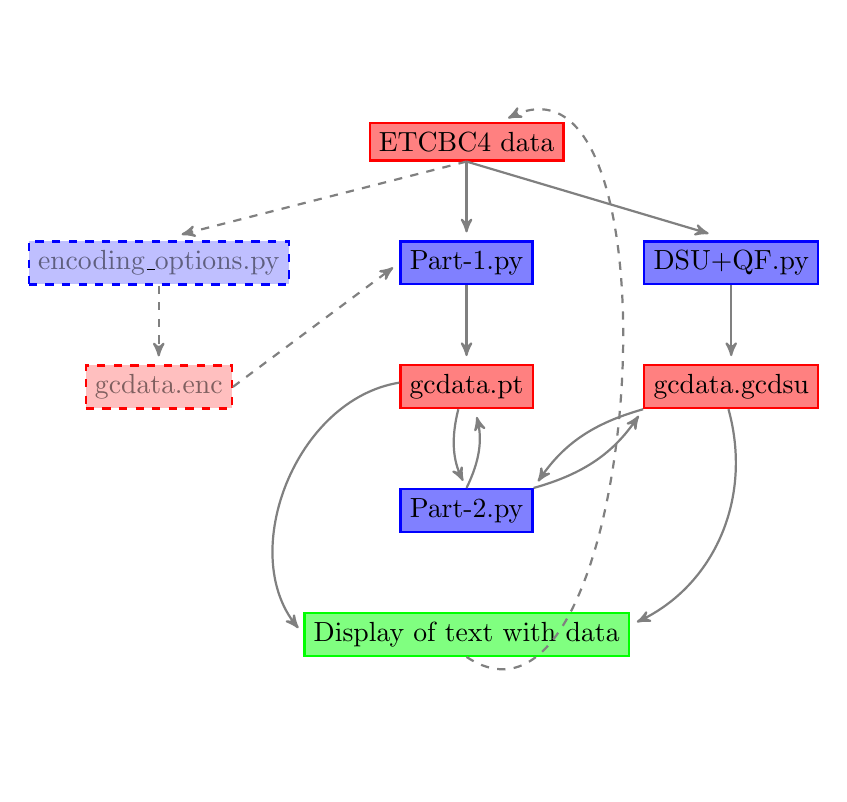
\begin{tikzpicture}[outline/.style={draw=#1,thick,fill=#1!50},
>=stealth',thick,black!50,text=black,
every new ->/.style={shorten >=.3cm}]
\centering

\node [outline=red] (input) {ETCBC4 data};
\node [outline=blue](part1) [below = of input]{Part-1.py};
\draw [shorten > =.1cm, ->] (input.south) -- (part1.north);
\node[outline=blue](qf) [below right = of input]{DSU+QF.py};
\draw [shorten > =.3cm, ->] (input.south) -- (qf.north);
\node[dashed, outline=blue, fill opacity =.5](enc) [below left = of input]{encoding\_options.py};
\draw [dashed, shorten > =.3cm, ->] (input.south) -- (enc.north);

\node [outline=red] (pt) [below=of part1]{gcdata.pt};
\draw [shorten > =.1cm, ->] (part1) -- (pt);

\node [dashed, outline=red, fill opacity =.5](enc2)[below = of enc]{gcdata.enc};
\draw [dashed, shorten > =.1cm, ->] (enc.south) -- (enc2.north);
\draw [dashed, shorten > =.1cm, ->] (enc2.east) -- (part1.west);

\node [outline=red] (gcdsu) [below=of qf]{gcdata.gcdsu};
\draw [shorten > =.1cm, ->] (qf.south) -- (gcdsu.north);
\node [outline=blue] (part2) [below = of pt] {Part-2.py};
\draw [shorten > =.1cm, ->] (pt) to [bend right = 20] (part2.north);
\draw [shorten > =.1cm, ->] (part2.north) to [bend right = 20] (pt);
\draw [shorten > =.1cm, ->] (gcdsu.south west) to [bend right = 20] (part2.north east);
\draw [shorten > =.1cm, ->] (part2.north east) to [bend right = 20] (gcdsu.south west);

\node [outline=green](show)[below = of part2]{Display of text with data};
\draw [shorten > =.1cm, ->] (gcdsu) to [bend left = 40] (show);
\draw [shorten > =.1cm, ->] (pt) to [bend right = 60] (show.west);
\draw [dashed, shorten > =.1cm, ->] (show.south) to [bend right = 120] (input);
\end{tikzpicture}

\chapter{Packages and LAF data that have to be loaded for executing the scripts}

\begin{python}
#{{{ Import all important libraries
import os, sys, time
if not '/projects/1fdd6b0b-5199-4b0e-9f7f-7759af4a5e7a/.local/lib/python3.4/site-packages/' in sys.path:
    sys.path.append('/projects/1fdd6b0b-5199-4b0e-9f7f-7759af4a5e7a/.local/lib/python3.4/site-packages/')
import collections
import random
import laf
from laf.fabric import LafFabric
import etcbc
from etcbc.preprocess import prepare
from etcbc.lib import Transcription, monad_set
from etcbc.trees import Tree
from etcbc.featuredoc import FeatureDoc
fabric = LafFabric()
tr = Transcription()

print("It works so far." )
#}}}
\end{python}

\begin{python}
#{{{ Load the API
API = fabric.load("etcbc4", "--", "feature-doc", {
    "xmlids": {"node": False, "edge": False},
    "features": ('''
            otype
            domain
            function
            g_cons
            g_cons_utf8
            g_lex
            g_lex_utf8
            g_nme
            g_nme_utf8
            g_pfm
            g_pfm_utf8
            g_prs
            g_prs_utf8
            g_uvf
            g_uvf_utf8
            g_vbe
            g_vbe_utf8
            g_vbs
            g_vbs_utf8
            g_word
            g_word_utf8
            gn
            lex
            lex_utf8
            ls
            nme
            nu
            number
            pdp
            pfm
            prs
            ps
            rela
            sp
            st
            tab
            trailer_utf8
            txt
            typ
            uvf
            vbe
            vbs
            vs
            vt
            book
            chapter
            label
            verse
    ''',""),
    "primary": False,
    "prepare": prepare,
})
exec(fabric.localnames.format(var='fabric'))
#}}}
\end{python}

\begin{python}
#{{{ Stuff necessary to load parents relationships
type_info = (
    ("word", ''),
    ("subphrase", 'U'),
    ("phrase", 'P'),
    ("clause", 'C'),
    ("sentence", 'S'),
)
type_table = dict(t for t in type_info)
type_order = [t[0] for t in type_info]

pos_table = {
    'adjv': 'aj',
    'advb': 'av',
    'art': 'dt',
    'conj': 'cj',
    'intj': 'ij',
    'inrg': 'ir',
    'nega': 'ng',
    'subs': 'n',
    'nmpr': 'n-pr',
    'prep': 'pp',
    'prps': 'pr-ps',
    'prde': 'pr-dem',
    'prin': 'pr-int',
    'verb': 'vb',
}

ccr_info = {
    'Adju': ('r', 'Cadju'),
    'Attr': ('r', 'Cattr'),
    'Cmpl': ('r', 'Ccmpl'),
    'CoVo': ('n', 'Ccovo'),
    'Coor': ('x', 'Ccoor'),
    'Objc': ('r', 'Cobjc'),
    'PrAd': ('r', 'Cprad'),
    'PreC': ('r', 'Cprec'),
    'Resu': ('n', 'Cresu'),
    'RgRc': ('r', 'Crgrc'),
    'Spec': ('r', 'Cspec'),
    'Subj': ('r', 'Csubj'),
    'NA':   ('n', 'C'),
}

tree_types = ('sentence', 'clause', 'clause_atom', 'phrase', 'subphrase', 'word')
(root_type, leaf_type, clause_type) = (tree_types[0], tree_types[-1], 'clause')
ccr_table = dict((c[0],c[1][1]) for c in ccr_info.items())
ccr_class = dict((c[0],c[1][0]) for c in ccr_info.items())

root_verse = {}
root_clause_atom = {}

for n in NN():
    otype = F.otype.v(n)
    if otype == "book" and F.etcbc4_sft_book.v(n) != "Genesis":
        break
    elif otype == "chapter" and int(F.etcbc4_sft_chapter.v(n)) > 5:
        break
    elif otype == "verse": cur_verse = F.label.v(n)
    elif otype == "clause_atom":
        root_verse[n] = cur_verse
        cur_clause_atom = F.etcbc4_ft_number.v(n)
    elif otype == "word":
        root_verse[n] = cur_verse
        root_clause_atom[n] = cur_clause_atom
#        print(list(C.parent.v(n)))

tree = Tree(API, otypes = tree_types,
     clause_type=clause_type,
     ccr_feature='rela',
     pt_feature='typ',
     pos_feature='sp',
     mother_feature = 'mother',
     )
#tree.restructure_clauses(ccr_class)
results = tree.relations()
parent = results['eparent']
sisters = results['sisters']
children = results['echildren']
elder_sister = results['elder_sister']
print("Ready for processing") # Was msg()
#}}}
\end{python}

\begin{python}
#{{{ Import the helper functions
def give_me_your_words(n):
        global F
        if F.etcbc4_db_otype.v(n) == 'word':
                return [n]
        else:
            list_of_word_lists = [give_me_your_words(c) for c in children[n]]
            return [item for sublist in list_of_word_lists for item in sublist]

def get_text_of_word_list(word_list):
        global F
        return ' '.join(map(F.etcbc4_ft_g_cons_utf8.v, word_list))

def get_cons_of_word_list(word_list):
        global F
        return ' '.join(map(F.etcbc4_ft_g_cons.v, word_list))

def give_me_your_parents_up_to(node, parent_type='clause', limit=19):
    # This function is very dangerous. If you feed it something larger than a clause, stuff explodes.
        global parent
        if limit < 0:
                return []
        if not n in parent:
                return ["not in parent"]
        p = parent[node]
        if F.etcbc4_db_otype.v(p) == parent_type:
                return [p]
        else:
                return [p] + give_me_your_parents_up_to(p, parent_type, limit-1)

suffix_dict = {
'W'   : { 'ps' : 'p3', 'nu' : 'sg', 'gn' : 'm' },
'K'   : { 'ps' : 'p2', 'nu' : 'sg', 'gn' : 'm' },
'J'   : { 'ps' : 'p1', 'nu' : 'sg', 'gn' : 'unknown' },
'M'   : { 'ps' : 'p3', 'nu' : 'pl', 'gn' : 'm' },
'H'   : { 'ps' : 'p3', 'nu' : 'sg', 'gn' : 'f' },
'HM'  : { 'ps' : 'p3', 'nu' : 'pl', 'gn' : 'm' },
'KM'  : { 'ps' : 'p2', 'nu' : 'pl', 'gn' : 'm' },
'NW'  : { 'ps' : 'p1', 'nu' : 'pl', 'gn' : 'unknown' },
'HW'  : { 'ps' : 'p3', 'nu' : 'sg', 'gn' : 'm' },
'NJ'  : { 'ps' : 'p1', 'nu' : 'sg', 'gn' : 'unknown' },
'K='  : { 'ps' : 'p2', 'nu' : 'sg', 'gn' : 'f' },
'HN'  : { 'ps' : 'p3', 'nu' : 'pl', 'gn' : 'f' },
'H='  : { 'ps' : 'p3', 'nu' : 'sg', 'gn' : 'unknown' },
'MW'  : { 'ps' : 'p3', 'nu' : 'pl', 'gn' : 'm' },
'N'   : { 'ps' : 'p3', 'nu' : 'pl', 'gn' : 'f' },
'KN'  : { 'ps' : 'p2', 'nu' : 'pl', 'gn' : 'f' },
}

def insert_dict_in_db(cursor, table, values):
        columns = ', '.join(values.keys())
        placeholders = ':'+', :'.join(values.keys())
        query = 'INSERT INTO %s (%s) VALUES (%s)' % (table, columns, placeholders)
#        print(query)
        cursor.execute(query, values)
#}}}
\end{python}

\chapter{DSU+QF.py}
\lstset{language=python,basicstyle=\ttfamily}

\begin{multicols}{2}
In this task I want to extract information from the ETCBC database + ask for user-input about DSU's and QF's + put it into an SQLite-table.
A DSU is a Direct Speech Unit, and a QF is a Quotative Frame.

\textbf{WARNING:} DSU's are found on the basis of \mi{text_type}s of \mi{clause_atom}s as stored in the ETCBC database. However, testing shows that these are not 100\% correct and will need improvement.

\textbf{WARNING2:} This task assumes that a DSU ends when the embedding (number of \mi{Q}'s in the \mi{text_type} of a \mi{clause_atom}) decreases.
However, it might very well be possible that various DSU's follow each other on the same level of embedding without intervening lower-\mi{Q} \mi{clause_atom}s.
At the moment these cases will not be detected by this script!
\end{multicols}

\begin{python}
#{{{ Create an SQLite-table with a row for every QF + DSU, and columns for useful information about these DSU's.
import sqlite3
db = sqlite3.connect('gcdata.sqlite')
c = db.cursor()

create_table_query = open('gcdsu.sql').read()

c.execute(create_table_query)

db.commit()
#}}}
\end{python}

\begin{multicols}{2}
Now we want to determine which \mi{clause_atom_number}s constitute QF's, and gather \mi{user_input} about them.
\begin{itemize}
 \item Show 4 clauses before DSU + first 4 clauses of DSU itself, all with \mi{clause_atom_number} and \mi{g_consonants}.
 \item Ask for block of \mi{clause_atom}s before DSU:
 \begin{itemize}
    \item Which \mi{clause_atom}s (if any) are QF
    \item What ``MySp" is. Can be any name
    \item What ``QFSp" is. Can be anything, or \mi{NULL}
    \item What ``QFSptype" is. Options: \mi{Noun}, \mi{Noun_phrase}, \mi{Name}, \mi{Name_phrase}, \mi{Pers_pronoun}, \mi{Suffix}, \mi{Verb}
    \item What ``MyAd" is. Can be any name
    \item What ``QFAd" is. Can be anything, or \mi{NULL}
    \item What ``QFAdtype" is. Options: \mi{Noun}, \mi{Noun_phrase}, \mi{Name}, \mi{Name_phrase}, \mi{Pers_pronoun}, \mi{Suffix}, \mi{Verb}
    \item What ``QFAdprep" is
    \item What ``QFplus" is. Can be anything, or \mi{NULL}
    \item What ``QFplustype" is. Can be something like \mi{Time} or \mi{Space}, or \mi{NULL}
  \end{itemize}
\end{itemize}
\end{multicols}

\begin{python}
#{{{ Verbs
def verbs(QFClANrs):
    QFverb,QFverbspeech,QFLMR = [],[],"No"
    for x in QFClANrs:
        for y in get_text_of_word_list(give_me_your_words(x)):
            if F.etcbc4_ft_sp.v(y) == "verb":
                QFverb.append(y)
                if F.etcbc4_ft_ls.v(y) == "quot":
                    QFverbspeech.append(y)
                    if F.etcbc4_ft_lex.v(y) == ">MR[" and F.etcbc4_ft_vt.v(y) == "infc":
                        QFLMR = "Yes"
    return(','.join(str(x) for x in QFverb),','.join(str(x) for x in QFverbspeech),QFLMR)

#}}}
\end{python}

\begin{python}
#{{{ Process_DSU
def process_DSU(ClANrs, potential_QF, place,prev_context,context,level):
    DSUdata = {}
    print(place)
    print("Potential QF:")  # Show the clause_atom_numbers of potential_QF with their text
    for x in potential_QF:
        print('{0:<8} {1:>35} {2} {3:<35}'.format(x, get_text_of_word_list(give_me_your_words(x))," | ", get_cons_of_word_list(give_me_your_words(x))))
    print("Start of DSU:")  # Show the first clause_atom_numbers and text of the DSU
    for y in ClANrs[:3]:
        print('{0:<8} {1:>35} {2} {3:<35}'.format(y, get_text_of_word_list(give_me_your_words(y))," | ",get_cons_of_word_list(give_me_your_words(y))))
    print("-"*20)
    DSUdata["a"] = place
    DSUdata["Level"] = level
#    DSUdata["ClANrs"] = ','.join(str(x) for x in ClANrs)
    DSUdata["ClANrs"] = repr(ClANrs)
    DSUdata["Con1"] = prev_context
    DSUdata["Con2"] = context
    DSUdata["QFClANrs"] = input("Clause_atoms that are indeed QF (type comma-separated numbers): ") or ""
    DSUdata["QFverb"],DSUdata["QFverbspeech"],DSUdata["QFLMR"] = verbs(DSUdata["QFClANrs"])
    DSUdata["QFSp"] = input("QFSp: ") or None
    DSUdata["QFSptype"] = input("QFSptype (1=Noun, 2=Noun_phrase, 3=Name, 4=Name_phrase, 5=Pers_pronoun, 6=Other_pronoun, 7=Suffix, 8=Verb): ") or None
    DSUdata["MySp"] = repr(input("MySp: ").split(",")) or None
    DSUdata["QFAd"] = input("QFAd: ") or None
    DSUdata["QFAdtype"] = input("QFAdtype (1=Noun, 2=Noun_phrase, 3=Name, 4=Name_phrase, 5=Pers_pronoun, 6=Other_pronoun, 7=Suffix, 8=Verb): ") or None
    DSUdata["QFAdprep"] = input("QFAdprep: ") or None
    DSUdata["MyAd"] = repr(input("MyAd: ").split(",")) or None
    DSUdata["QFplus"] = input("QFplus: ") or None
    DSUdata["QFplustype"] = input("QFplustype: ") or None
    DSUdata["Start_node"] = ClANrs[0]
    DSUdata["DSUtag"] = str(DSUdata["Start_node"]) + str(DSUdata["Level"])
    if DSUdata["QFClANrs"] != "":
        DSUdata["QF"] = "Yes"
    elif DSUdata["QFClANrs"] == "":
        DSUdata["QF"] = "No"
    insert_dict_in_db(c, "gcdsu", DSUdata)

#}}}
\end{python}

\begin{python}
#{{{ Main function
def main_loop():
    ClANrs =       [[],[],[],[],[],[],[],[]]
    potential_QF = [[],[],[],[],[],[],[],[]]
    pot_QF = []
    context = ""
    prev_context = ["","","","","","","",""]

    place = None
    places =       ["","","","","","","",""]
    level = 0
    completed = False
    check_node = ""

    for node in NN():
        otype = F.etcbc4_db_otype.v(node)

        if otype == "book" and F.etcbc4_sft_book.v(node) != "Genesis":
            break
        elif otype == "chapter":
            if int(F.etcbc4_sft_chapter.v(node)) < 2:    # Prevent re-doing already completed chapters
                completed = True
            elif int(F.etcbc4_sft_chapter.v(node)) > 3:    # Set a limit on the amount of data dealt with this time
                break
            else:
                completed = False

        elif otype == "verse" and completed == False:
            place = F.etcbc4_sft_label.v(node)
        elif otype == "clause" and completed == False:
            prev_level = level
            level = F.etcbc4_ft_txt.v(node).count("Q")      # Determine level by parsing text_type data
            previous_context = context
            context = F.etcbc4_ft_txt.v(node)

        elif otype == "clause_atom" and completed == False:
            pot_QF.append(node)     # Update pot_QF
            if len(pot_QF) > 5:
                del pot_QF[0]       # Keep length of pot_QF reasonable
            if level > 0:           # At least one DSU under construction
                for i in range(1,(level+1)):
                    ClANrs[level].append(node)   # For all DSU's under construction, add current ClANr to list of ClANrs
            if prev_level < level:                  # Start of new DSU
                places[level] = place               # Store starting place of new DSU
                potential_QF[level] = pot_QF[:-1]   # Store potential QF of new DSU
                prev_context[level] = previous_context    # Store context (preceding text_type)

            elif prev_level > level:                # End of one or more DSU's
                for j in range((level+1),(prev_level+1)): # Process the DSU's that end here
                    check_node = str(ClANrs[j][0])
                    c.execute("SELECT EXISTS (SELECT * FROM gcdsu WHERE Start_node = " + check_node + ");") # Check whether DSU is not yet saved in database
                    result = c.fetchone()
                    if result == (0,):
                        process_DSU(ClANrs[j], potential_QF[j],places[j],prev_context[j],context,j)
                    ClANrs[j], potential_QF[j], places[j], prev_context[j] = [],[],"",""    # Delete all stored data

#}}}
\end{python}

\begin{python}
#{{{ Execute main loop
main_loop()
#}}}

#{{{ Wrap up the database connection
db.commit()
c.close()
#}}}
\end{python}

\chapter{encoding\_options.py}
\chapter{Part-1.py}
\begin{python}
#{{{ Setup the database stuff
import sqlite3

db = sqlite3.connect('gcdata.sqlite')
c = db.cursor()

create_table_query = open("pt.sql").read()
c.execute(create_table_query)

db.commit()

#}}}
\end{python}

\begin{python}
#{{{ Find fitting info about types and functions
def types_functions(node,node_type,Clause,ClANr,Phrase,PhANr,SPhNr,WNr,Data):
        if Data["Nodetype"] == "6":                # On extensive nodetypes, info on smaller items makes no sense
            ClANr,PhANr,SPhNr,WNr) = (0,0,0,0)
        elif Data["Nodetype"] == "5":
            (PhANr,SPhNr,WNr) = (0,0,0)
        elif Data["Nodetype"] in ("3","4"):
            WNr = 0
        Data["ClANr"] = ClANr                      # Insert data on numbers
        Data["PhANr"] = PhANr
        Data["SPhNr"] = SPhNr
        Data["WNr"] = WNr

        Data["Cltype"] = F.etcbc4_ft_typ.v(Clause) # Insert data on types and function
        Data["Phtype"] = F.etcbc4_ft_typ.v(Phrase)
        Data["Phfunc"] = F.etcbc4_ft_function.v(Phrase)
        if Data["Nodetype"] == "6":                # On extensive nodetypes, info on smaller items makes no sense
            Data["Cltype"] = ""
        if Data["Nodetype"] in ("5","6"):
            Data["Phtype"] = ""
            Data["Phfunc"] = ""

        if 1< int(Data["Nodetype"]) < 4:           # Word nodes have a Part of Speech, and sometimes a Lexical Set too
            Data["PartSpeech"] = F.etcbc4_ft_sp.v(node)
            Data["Lexset"] = F.etcbc4_ft_ls.v(node)
        else:
            Data["PartSpeech"] = input("Part of speech: ")
            Data["Lexset"] = input("Lexical set: ")

        # Encoding options as stored in gcdata.enc
#        Data["Enc_opt"] = c.execute("select Enc_options from enc where Cl_type=:Cltype and Ph_func=:Phfunc", {"Cltype":Data["Cltype"],"Phfunc":Data["Phfunc"]})
#        Data["Enc_opt_coded"] = c.execute("select Enc_options_coded from enc where Cl_type=:Cltype and Ph_func=:Phfunc", {"Cltype":Data["Cltype"],"Phfunc":Data["Phfunc"]})
#        coding = Data["PartSpeech"]
#        if coding == "verb":
#            prom1 = 1
#        elif coding == "suffix":
#            prom1 = 2
#        elif z == "prps":
#            prom1 = 3
#        elif z == "prde":
#            prom1 = 4
#        elif z in ("subs","nmpr","adjv"):
#            prom1 = 5
#        elif Data["Nodetype"] in ("4","5","6"):
#            prom1= 6
#        Data["Prom"] = eval(Data["Enc_opt_coded"]).index(prom1)

        function = F.etcbc4_ft_function.v(Phrase)
        if Data["Nodetype"] in ("1", "2", "3", "4"):    # F.etcbc4_ft_function.v(node) only applies to phrase level (or lower)
            if function in ("ExsS","IntS","ModS","NCoS","PrcS","PreS") and Data["Nodetype"] == "1":
                Data["Role"] = "Subject"
            elif function in ("PreO","PtcO") and Data["Nodetype"] == "1":
                Data["Role"] = "Object"
            elif Data["Nodetype"] == "1" or F.etcbc4_ft_rela.v(SPhNr) == "rec":
                Data["Role"] = input("Grammatical role / function:" + "rec") or "rec"
            else:
                Data["Role"] = input("Grammatical role / function: " + function ) or function
        else:
            Data["Role"] = input("Grammatical role / function: ")

#}}}
\end{python}

\begin{python}
#{{{ Find potential reference levels + ask for some user-input + feed data about reference to SQLite
def ask_potential_ref(place, node, node_type, Clause, ClANr, Phrase, PhANr, SPhNr, WNr):
        Data = {}
        print("-"*20)
        print(place)
        print("Clause_atom:", get_cons_of_word_list(give_me_your_words(ClANr)))
        if node_type == "word":
                lijstje = [node] + give_me_your_parents_up_to(node)
        elif node_type == "suffix":
                lijstje = [node] + [node] + give_me_your_parents_up_to(node)
        for l in lijstje:
                print('{0: <8} {1: <8} {2: >15} {3} {4:<15}'.format(l, F.etcbc4_db_otype.v(l), get_text_of_word_list(give_me_your_words(l))," | ",get_cons_of_word_list(give_me_your_words(l))))
        Data["a"] = place
        Data["Node"] = node
        Data["Emb"] = F.etcbc4_ft_tab.v(ClANr)
        Data["Des"] = F.etcbc4_ft_g_cons.v(node)
        Data["Nodetype"] = input("Which node_type do you want to store? (1=Part_suffix, 2=Part_word, 3=Part_subphrase, 4=Part_phrase, 5=Part_clause, 6=Part_sentence): ")
        Data["Destype"] = input("What is the designation type? (1=Noun, 2=Noun_phrase, 3=Name, 4=Name_phrase, 5=Pers_pronoun, 6=Demonstr_pronoun, 7=Suffix, 8=Verb): ")
        Sub-data = ""
        if F.etcbc4_ft_rela.v(Clause) == "Attr":
            Sub-data.append("Attr")
        if Data["Nodetype"] == "3" and F.etcbc4_ft_rela.v(SPhNr) == "rec":
            Sub-data.append("rec")
        elif F.etcbc4_ft_rela.v(node) == "REG":
            Sub-data.append("Sub1")
        if Sub-data == "":
            Sub-data = "No"
        Data["Sub"] = input("Is this a sub-participant? Default" Sub-data) or Sub-data
        Data["Name"] = input("What is the name of the referent? : ")
        Data["Anim"] = input("1=Animate, 2=Non-animate: ")
        if Data["Anim"] == "2":
            Data["Human"] = "None"
        elif Data["Anim"] == "1":
            Data["Human"] = input("1=Human (or divine), 2=Non-human")
        Data["Col"] = input("Is the participant an individual (1), collective (2) or an individual in a compound design (3)?")
        if Data["Col"] == "2" or Data["Col"] == "3":
            Data["Referents"] = input("Contextually relevant referents that are part of Name: ")
            Data["ColPart"] = input("Contextually relevant collective of which Name is part: ") or None
        else:
            Data["Referents"] = None
            Data["ColPart"] = input("Contextually relevant collective of which Name is part: ") or None
        if node_type == "word":
            Data["P"] = F.etcbc4_ft_ps.v(node)
            Data["N"] = F.etcbc4_ft_nu.v(node)
            Data["G"] = F.etcbc4_ft_gn.v(node)
        elif node_type == "suffix":
            Data["P"] = suffix_dict[F.etcbc4_ft_prs.v(node)]['ps']    # Since the suffix_features are not yet available in the ETCBC database, we extract them from a dictionary based on surface consonants
            Data["N"] = suffix_dict[F.etcbc4_ft_prs.v(node)]['nu']
            Data["G"] = suffix_dict[F.etcbc4_ft_prs.v(node)]['gn']
        Data["Tag"] = Data["a"].rjust(15,'') + "_" + str(ClANr).rjust(9,'0') + "_" + str(PhANr).rjust(9,'0') + "_" + str(WNr).rjust(9,'0') + "_" + str(Data["Nodetype"])

        insert_dict_in_db(c,"pt",Data)
		Done = input("Done with this reference! If not, type 'No'") or None
			if Done == "No":
				ask_potential_ref(place, node, node_type, Clause, ClANr, Phrase, PhANr, WNr)
    
#}}}
\end{python}

\begin{python}
#{{{ Record some statistics and filter potential participant references
DSU = False
completed = False

limit = 0
for node in NN():
    otype = F.etcbc4_db_otype.v(node)
    if otype == "book" and F.etcbc4_sft_book.v(node) != "Genesis":
        break
    elif otype == "chapter":
        if int(F.etcbc4_sft_chapter.v(node)) < 1:    # Prevent re-doing already completed chapters
            completed = True
        elif int(F.etcbc4_sft_chapter.v(node)) > 3:    # Set a limit on the amount of data dealt with this time
            break
        else:
            completed = False
    elif otype == "verse" and completed == False:
        place = F.etcbc4_sft_label.v(node)
    elif otype == "clause" and completed == False:
        DSU = (F.etcbc4_ft_txt.v(node).count("Q") > 0)    # If the text_type contains a Q, we consider the clause as Direct Speech
        Clause = node
    elif otype == "clause_atom" and completed == False:
        ClANr = node
        PhANr = 0
    elif otype == "phrase" and completed == False:
        Phrase = node
        SPhNr = None
    elif otype == "phrase_atom" and completed == False:
        PhANr = node
    elif otype == "subphrase":
        SPhNr = node
    elif F.etcbc4_db_otype.v(node) == "word" and DSU == True and completed == False:
        WNr = node
        check_node = str(node)
        c.execute("SELECT count(*) FROM pt WHERE Node = " + check_node + ";") # Check whether reference is not yet saved in database
        result = c.fetchone()
        if result == (0,) or (result == (1,) and not (F.etcbc4_ft_prs.v(node) in ("absent","n/a")) and not (F.etcbc4_ft_ps.v(node) in ("unknown", "NA") and F.etcbc4_ft_nu.v(node) in ("unknown","NA") and F.etcbc4_ft_gn.v(node) in ("unknown","NA"))):    # Apparently reference is not yet saved in database (in case of a suffix, word may be saved already)
            if not (F.etcbc4_ft_ps.v(node) in ("unknown", "NA") and F.etcbc4_ft_nu.v(node) in ("unknown","NA") and F.etcbc4_ft_gn.v(node) in ("unknown","NA")):    # Check whether node is a potential reference by checking features person, number, gender.
                ask_potential_ref(place, node, "word", Clause, ClANr, Phrase, PhANr, SPhNr, WNr)
            if not F.etcbc4_ft_prs.v(node) in ("absent","n/a"):
                ask_potential_ref(place, node, "suffix", Clause, ClANr, Phrase, PhANr, SPhNr, WNr)
#}}}
\end{python}

\begin{python}
#{{{ Commit and close the database
db.commit()
db.close()
#}}}
\end{python}

\chapter{Part-2.py}
\begin{python}
#{{{ Load database
import sqlite3

db = sqlite3.connect('gcdata.sqlite')
c = db.cursor()
#}}}
\end{python}

From gcdata.gcdsu we want to extract the \mi{DSU_Tag}, so that we can easily see
whether various participant references occur in the same DSU or in a different one.
For each DSU we create a dictionary item with its \mi{Tag}, \mi{place} and \mi{clause_atom_numbers}.
We then check of which DSU the \mi{clause_atom_number} of the current participant
reference is part, and store its \mi{Tag} in the column \mi{DSU}.

\begin{python}
#{{{ Assign DSU and Level
DSU_Tags = list(c.execute("select DSUtag,Level,ClANrs from gcdsu"))
pts = list(c.execute("select Tag,a,ClANr from pt where DSU is null or DSU = ''"))

DSU = {}

for (Tag,a,ClANr) in pts:
    for (DSUtag,Level,ClANrs) in DSU_Tags:
        if str(ClANr) in ClANrs.split(","):
            c.execute("update pt set DSU=:DSUtag,Level=:Level where a=:a and ClANr=:ClANr", {"DSUtag":DSUtag,"Level":Level,"a":a,"ClANr":str(ClANr)})
            DSU[Tag] = DSUtag

#}}}
\end{python}

\begin{python}
#{{{ Feed participants back to DSU (follows on previous block)
parts = {}

for (DSUtag,Level,ClANrs) in DSU_Tags:
    parts[DSUtag] = list(c.execute("select Part from gcdsu where DSUtag=:DSUtag", {"DSUtag":DSUtag, }))[0][0]

for (Tag,a,ClANr) in pts:
    probable_parts = []
    ColPart = list(c.execute("select ColPart from pt where Tag=:Tag", {"Tag":Tag, }))[0][0]
    if ColPart == None:
        ColPart = []
    else:
        ColPart = eval(ColPart)
    Referents = list(c.execute("select Referents from pt where Tag=:Tag", {"Tag":Tag, }))[0][0]
    if Referents == None:
        Referents = []
    else:
        Referents = eval(Referents)
    Name = list(c.execute("select Name from pt where Tag=:Tag", {"Tag":Tag, }))[0][0]
    probable_parts = ColPart + Referents
    probable_parts.append(Name)
    if parts[DSU[Tag]] != None:
        probable_parts += eval(parts[DSU[Tag]])
    all_parts = list(set(probable_parts))
    parts[DSU[Tag]] = str(all_parts)
    c.execute("update gcdsu set Part=:all_parts where DSUtag=:DSUtag", {"all_parts":str(all_parts), "DSUtag":DSU[Tag]})

#}}}
\end{python}

In order to facilitate the combination of information between SQlite rows,
we assign a number to each participant reference, indicating how many times
this participant has been referred to, including the current reference.
Later on, we can then identify the \mi{Ref}-values by selecting values with the
same \mi{Name} and a \mi{Nr} that is 1 lower than the current \mi{Nr}.
A difficulty arises when a participant is referred to as part of a group,
e.g. ``God said to them...'' meaning both the man and the woman of \bibleverse{Gen}[1].
Therefore I provide two kinds of information:
\begin{itemize}
\item A \mi{Nr} that indicates the number of occurrences of exactly the same referent. This is relevant for \mi{Prev}-data and \mi{Ref}-data.
\item I mention the names of relevant referents that are included in other referents etc in the column \mi{Referents}, so that these can be counted and processed later on (e.g. to see how often someone is referred to in a particular DSU).
\end{itemize}
Another aspect that adds complexity, is the occurrence of sub-participants.
I do not count them in the column \mi{Nr}, but their name is stored in the columns
\mi{Name} and \mi{Referents}.


\begin{python}
#{{{ Assign Nr - new try
nrs_todo = list(c.execute("select Sub, Name, Tag, Nr from pt where Nr is null or Nr = ''"))  # Select all rows that need a Nr
nrs = {}    # Create dict for all relevant Names + their Nrs

for (Sub, Name, Tag, Nr) in nrs_todo:
    if Sub == "No":
        if Name in nrs:
            newnr = nrs[Name] + 1
        elif Name not in nrs:
            oldnr = list(c.execute("select Nr from pt where Name=:Name ORDER BY Tag DESC LIMIT 1", {"Name":Name,}))
            if oldnr == [] or oldnr[0][0] == '':
                newnr = 1
            else:
                newnr = int(oldnr[0][0]) + 1
        nrs[Name] = newnr
        c.execute("update pt set Nr=:newnr where Tag=:Tag", {"newnr":newnr, "Tag":Tag})
#}}}
\end{python}

Below we do a for-loop over all rows in gcdata.pt that still miss certain data,
and update them with information about the preceding reference to this participant (\mi{Ref}),
the previous reference (irrespective of the participant) (\mi{Prev}) and the first reference
to this participant (\mi{1}).

We repeat the process for other information. Putting all these columns in one
for-loop would overload them and make the code unclear.

\begin{python}
#{{{ Update Ref, Prev and *1-data
all_tags = list(c.execute("select Tag from pt ORDER BY Tag"))
todo = list(c.execute("select Tag,Name,Nr from pt where RefNode is null or RefNode = ''"))

for (Tag,Name,Nr) in todo:
    Refdata = list(c.execute("select DSU, a, ClANr, PhANr, Node, Nodetype, WNr from pt where Name=:Name ORDER BY Tag DESC LIMIT 1", {"Name":Name, })) # Ref-data
    c.execute("update pt set RefDSU=:DSU, Refa=:a, RefClANr=:ClANr, RefPhANr=:PhANr, RefNode=:Node, RefNodetype=:Nodetype, RefWNr =:WNr where Name=:Name and Nr=:Nr",{"DSU":Refdata[0][0],"a":Refdata[0][1],"ClANr":Refdata[0][2],"PhANr":Refdata[0][3],"Node":Refdata[0][4],"Nodetype":Refdata[0][5],"WNr":Refdata[0][6],"Name":Name,"Nr":Nr}) 
    Onedata = list(c.execute("select DSU, a, ClANr, PhANr, Node, Nodetype, WNr from pt where Name=:Name ORDER BY Tag LIMIT 1", {"Name":Name, })) # *1-data
    c.execute("update pt set DSU1=:DSU, a1=:a, ClANr1=:ClANr, PhANr1=:PhANr, Node1=:Node, Nodetype1=:Nodetype, WNr1=:WNr where Name=:Name and Nr=:Nr",{"DSU":Onedata[0][0],"a":Onedata[0][1],"ClANr":Onedata[0][2],"PhANr":Onedata[0][3],"Node":Onedata[0][4],"Nodetype":Onedata[0][5],"WNr":Onedata[0][6],"Name":Name,"Nr":Nr}) 

    index = [y[0] for y in all_tags].index(Tag)  # Check the index of this row in the ordered list all_tags, in order to find the previous row = Prev_data 
    if index == 0:  # Apparently this is the first row of the table
        Prevdata = list(c.execute("select Name, DSU, a, ClANr, PhANr, Node, Nodetype, WNr from pt where Tag=:Tag",{"Tag":Tag, })) # Prev-data for first entry
    else:
        prev_Tag = all_tags[(index-1)][0]
        Prevdata = list(c.execute("select Name, DSU, a, ClANr, PhANr, Node, Nodetype, WNr from pt where Tag=:prev_Tag",{"prev_Tag":prev_Tag, })) # Prev-data
    c.execute("update pt set PrevName =:PrevName, PrevDSU=:DSU, Preva=:a, PrevClANr=:ClANr, PrevPhANr=:PhANr, PrevNode=:Node, PrevNodetype=:Nodetype, PrevWNr =:WNr where Name=:Name and Nr=:Nr",{"PrevName":Name,"DSU":Prevdata[0][0],"a":Prevdata[0][1],"ClANr":Prevdata[0][2],"PhANr":Prevdata[0][3],"Node":Prevdata[0][4],"Nodetype":Prevdata[0][5],"WNr":Prevdata[0][6],"Name":Name,"Nr":Nr}) 

for (Tag,Name,Nr) in todo:
    Refdata = list(c.execute("select Con, Level, Emb, Des, Destype, Role, P, N, G, Lexset, PartSpeech from pt where Name=:Name ORDER BY Tag DESC LIMIT 1", {"Name":Name, })) # Ref-data
    c.execute("update pt set RefCon=:Con, RefLevel=:Level, RefEmb=:Emb, RefDes=:Des, RefDestype=:Destype, RefRole=:Role, RefP=:P, RefN=:N, RefG=:G, RefLexset=:Lexset, RefPartSpeech=:PartSpeech where Name=:Name", {"Con":Refdata[0][0],"Level":Refdata[0][1],"Emb":Refdata[0][2],"Des":Refdata[0][3],"Destype":Refdata[0][4],"Role":Refdata[0][5],"P":Refdata[0][6],"N":Refdata[0][7],"G":Refdata[0][8],"Lexset":Refdata[0][9],"PartSpeech":Refdata[0][10],"Name":Name})
    index = [y[0] for y in all_tags].index(Tag)  # Check the index of this row in the ordered list all_tags, in order to find the previous row = Prev_data 
    if index == 0:  # Apparently this is the first row of the table
        Prevdata = list(c.execute("select Con, Level, Emb, Des, Destype, Role, P, N, G, Lexset, PartSpeech from pt where Tag=:Tag",{"Tag":Tag, })) # Prev-data for first entry
    else:
        prev_Tag = all_tags[(index-1)][0]
        Prevdata = list(c.execute("select Con, Level, Emb, Des, Destype, Role, P, N, G, Lexset, PartSpeech from pt where Tag=:prev_Tag",{"prev_Tag":prev_Tag, })) # Prev-data
    c.execute("update pt set PrevCon=:Con, PrevLevel=:Level, PrevEmb=:Emb, PrevDes=:Des, PrevDestype=:Destype, PrevRole=:Role, PrevP=:P, PrevN=:N, PrevG=:G, PrevLexset=:Lexset, PrevPartSpeech=:PartSpeech where Tag=:Tag", {"Con":Prevdata[0][0],"Level":Prevdata[0][1],"Emb":Prevdata[0][2],"Des":Prevdata[0][3],"Destype":Prevdata[0][4],"Role":Prevdata[0][5],"P":Prevdata[0][6],"N":Prevdata[0][7],"G":Prevdata[0][8],"Lexset":Prevdata[0][9],"PartSpeech":Prevdata[0][10],"Tag":Tag})
#}}}
\end{python}

\end{document}
%sagemathcloud={"latex_command":"pdflatex -synctex=1 -shell-escape -interact=nonstopmode 'workflow.tex'"}
